\documentclass[journal,onecolumn]{IEEEtran}

\usepackage{graphicx}
\usepackage{amsmath}
\usepackage{amssymb}
\usepackage{booktabs}
\usepackage{hyperref}
\usepackage{float}
\usepackage{subcaption}
\usepackage[margin=1in]{geometry}
\usepackage{cite}

\title{E0 270(0): Assignment 2 \\ Logistic Regression \& Multi-Layer Perceptron}
\author{Shashank Sekhar\\SR No.\ 26156}
\date{}

\begin{document}

\maketitle

\begin{abstract}
This report covers my attempt of assignment 2 consisting of part 1:-logistic regression from scratch (using PyTorch) and part 2:- three MLP architectures on the breast cancer Wisconsin dataset. The logistic regression model hit 97.09\% accuracy on the test set with learning rate 0.1. Among the linear MLPs the linear baseline actually performed best at 97.67\% while the deep network (3 hidden layers) struggled to converge which turned out to be an interesting lesson about initialization sensitivity and vanishing gradients.
\end{abstract}

% ============================================================
\section{Data and Preprocessing}
% ============================================================

The Breast Cancer Wisconsin (Diagnostic) dataset has 569 samples and 30 features. The label is \texttt{diagnosis} (M = malignant, B = benign), which I encoded as 1 and 0 respectively. There are 357 benign and 212 malignant samples so there's some class imbalance but nothing extreme.

\begin{figure}[H]
    \centering
    \begin{subfigure}[b]{0.48\textwidth}
        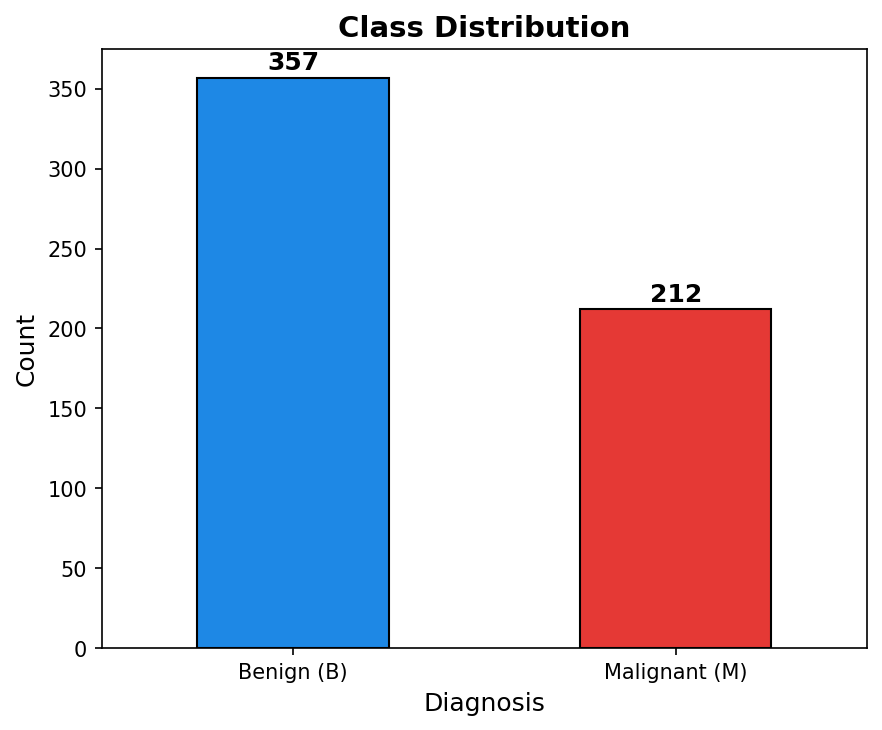
\includegraphics[width=\textwidth]{plots/eda/class_distribution.png}
        \caption{Class distribution.}
        \label{fig:class_dist}
    \end{subfigure}
    \hfill
    \begin{subfigure}[b]{0.48\textwidth}
        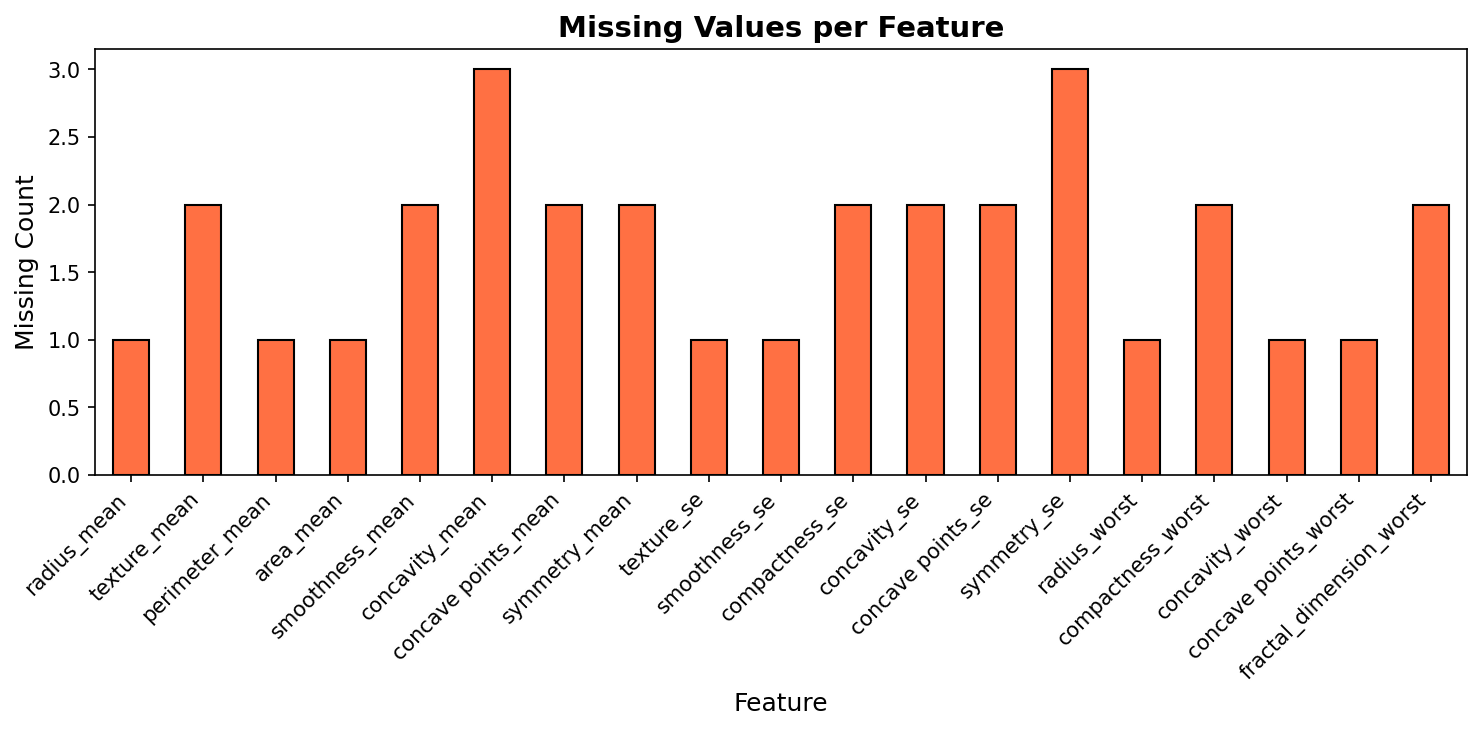
\includegraphics[width=\textwidth]{plots/eda/missing_values.png}
        \caption{Missing values per feature.}
        \label{fig:missing}
    \end{subfigure}
    \caption{Dataset overview.}
    \label{fig:eda_overview}
\end{figure}

I split the data into 397 training and 172 test samples using a 70/30 split (seed = 34). The dataset had 32 missing values scattered across a few columns (Figure~\ref{fig:missing}), so these were filled with feature-wise medians computed on the training split and then the same median applied to the test set.

Additionally, I applied z-score standardization (mean = 0, std = 1) using \texttt{StandardScaler}. This was done for faster convergence additionally it makes the learned weights directly comparable across features (which I require for the feature importance analysis later).

I deliberately didn't do any extra feature engineering like power transforms, no correlated feature removal, no dimensionality reduction in order to maintain feature interpretability. 

\begin{figure}[H]
    \centering
    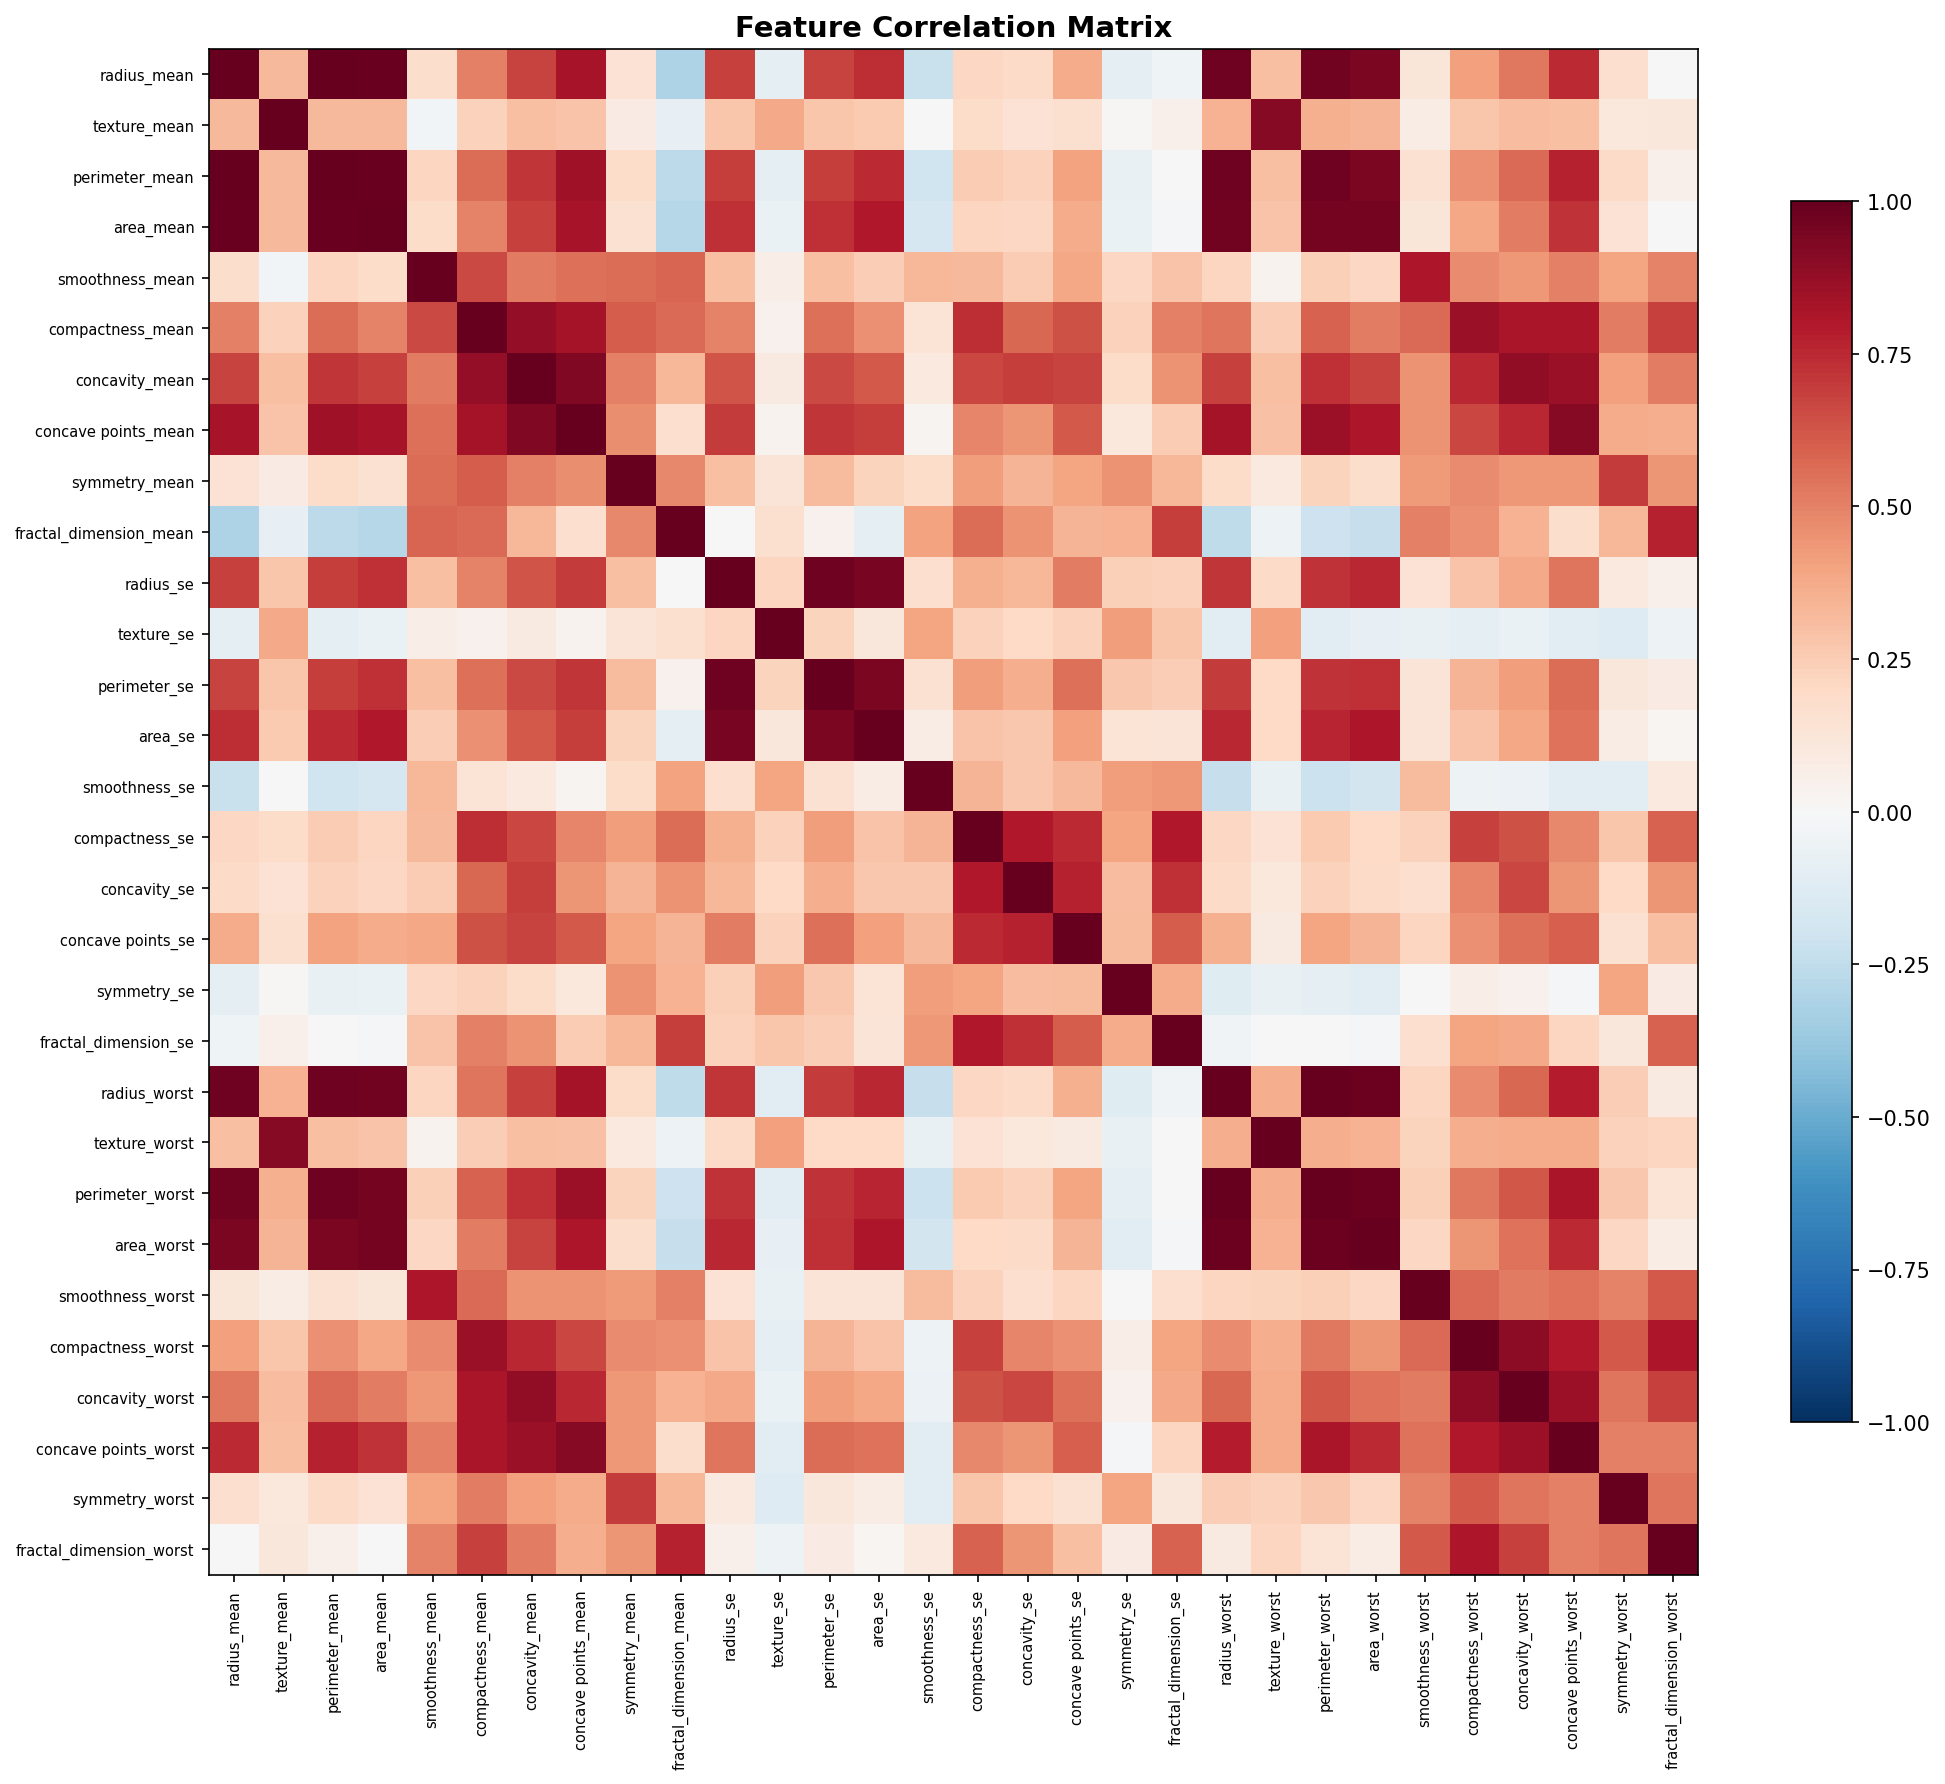
\includegraphics[width=0.8\textwidth]{plots/eda/correlation_heatmap.png}
    \caption{Feature correlation matrix. There's heavy multicollinearity -radius, perimeter, and area features are almost perfectly correlated ($r > 0.95$). I kept all features anyway since removing them would affect the weight interpretation the assignment asks for.}
    \label{fig:corr}
\end{figure}

% ============================================================
\section{Logistic Regression}
% ============================================================

\subsection{Model}

Logistic regression models the probability of the positive class as:
\begin{equation}
    P(y=1 \mid \mathbf{x}) = \sigma(\mathbf{w}^T\mathbf{x} + b) = \frac{1}{1 + e^{-(\mathbf{w}^T\mathbf{x} + b)}}
\end{equation}

The loss function is:
\begin{equation}
    \mathcal{L} = -\frac{1}{N}\sum_{i=1}^{N}\left[y_i \log(\hat{y}_i) + (1-y_i)\log(1-\hat{y}_i)\right]
\end{equation}
where $\hat{y}_i = \sigma(\mathbf{w}^T\mathbf{x}_i + b)$. I trained with SGD, no momentum or weight decay.

\subsection{Learning Rate Comparison}

As suggested in the problem statement, I trained the same with three learning rates: $\alpha \in \{0.1, 0.01, 0.001\}$, each for 1000 epochs. Figure~\ref{fig:lr_loss} shows how the loss curves look.

\begin{figure}[H]
    \centering
    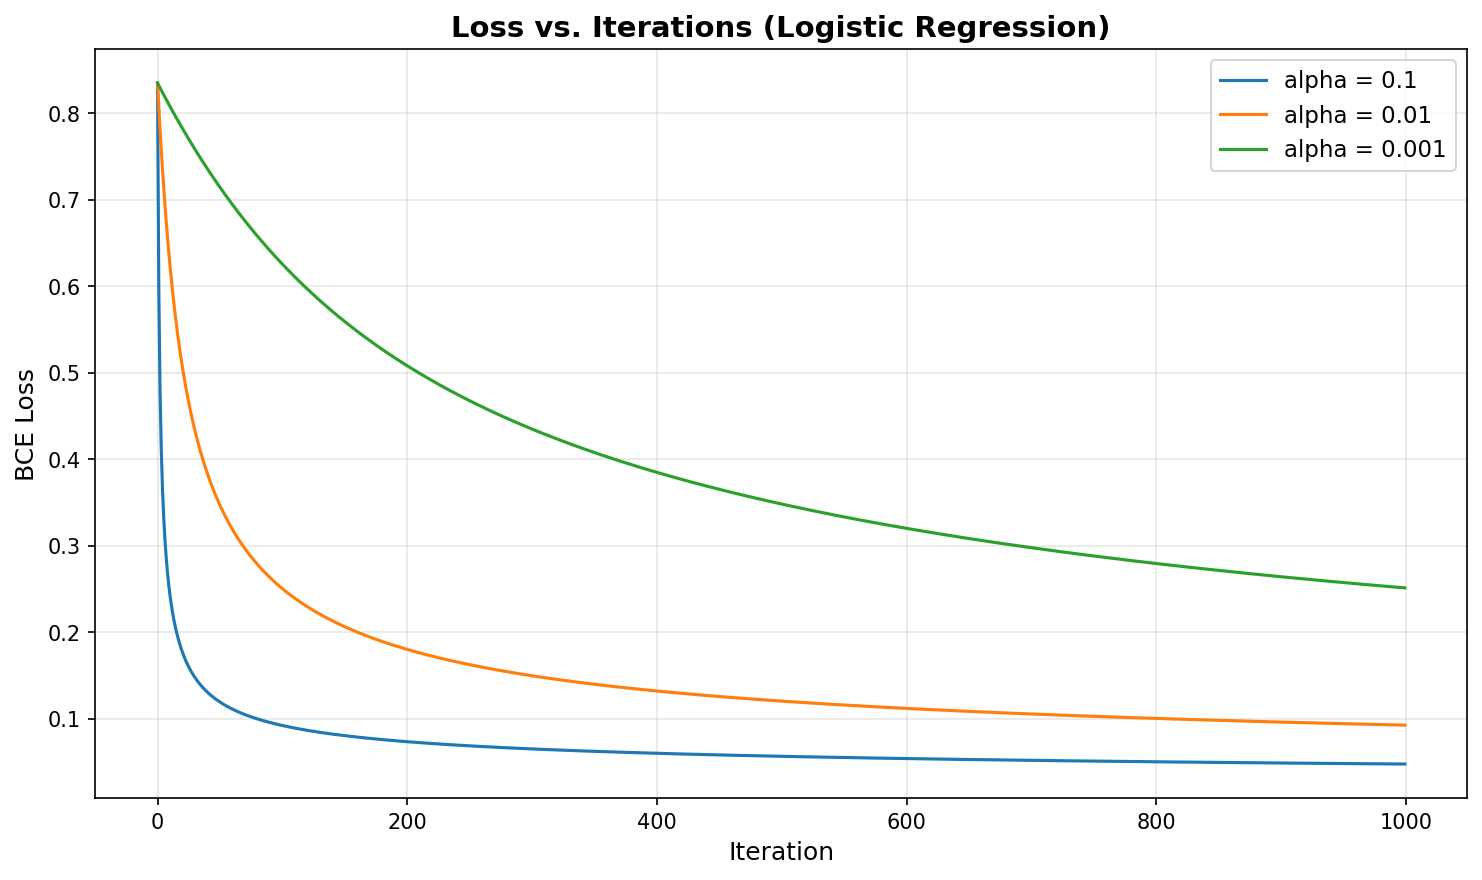
\includegraphics[width=0.75\textwidth]{plots/part1/lr_loss_vs_iterations.png}
    \caption{Loss vs.\ iterations for different learning rates.}
    \label{fig:lr_loss}
\end{figure}

$\alpha = 0.1$ converges the fastest.It's already below 0.1 by epoch 100 and basically flat after 400. $\alpha = 0.01$ gets there eventually but takes the full 1000 epochs to come close. $\alpha = 0.001$ is too slow and it's still at 0.25 after 1000 epochs and hasn't plateaued. I picked $\alpha = 0.1$ as the best model since it had the lowest final validation loss (0.1114).

\subsection{Test Set Evaluation}

\begin{table}[H]
\centering
\caption{Logistic Regression Test Results ($\alpha = 0.1$, 1000 epochs)}
\label{tab:lr_results}
\begin{tabular}{lc}
\toprule
\textbf{Metric} & \textbf{Value} \\
\midrule
Accuracy & 0.9709 \\
Precision & 0.9683 \\
Recall & 0.9531 \\
F1 & 0.9606 \\
ROC-AUC & 0.9876 \\
\bottomrule
\end{tabular}
\end{table}

For my best logistic regression model I got a 97.09\% accuracy with an AUC of 0.9876. Precision and recall are both above 0.95. There is a balance maintained between all three.

\subsection{Feature Importance}

Since the features are z-score normalized, the absolute value of each weight tells me how much that feature contributes to the decision boundary. Table~\ref{tab:feature_importance} shows the top 10.

\begin{table}[H]
\centering
\caption{Top 10 Features by $|$weight$|$}
\label{tab:feature_importance}
\begin{tabular}{clcc}
\toprule
\textbf{Rank} & \textbf{Feature} & \textbf{Weight} & $|\textbf{Weight}|$ \\
\midrule
1 & texture\_worst & 1.1152 & 1.1152 \\
2 & radius\_worst & 0.9282 & 0.9282 \\
3 & concavity\_worst & 0.8778 & 0.8778 \\
4 & smoothness\_worst & 0.8754 & 0.8754 \\
5 & concave points\_worst & 0.8462 & 0.8462 \\
6 & symmetry\_worst & 0.8220 & 0.8220 \\
7 & concave points\_mean & 0.7998 & 0.7998 \\
8 & radius\_mean & 0.7938 & 0.7938 \\
9 & area\_worst & 0.7759 & 0.7759 \\
10 & perimeter\_mean & 0.7227 & 0.7227 \\
\bottomrule
\end{tabular}
\end{table}

\texttt{Texture\_worst} contributed the most followed by \texttt{radius\_worst} and \texttt{concavity\_worst}. All the top weights are positive, meaning higher values push the prediction toward malignant.

The multicollinearity between features means that the individual weights can be a bit unstable. But the general picture that ``worst'' and shape-related features matter the most and is consistent.

\begin{figure}[H]
    \centering
    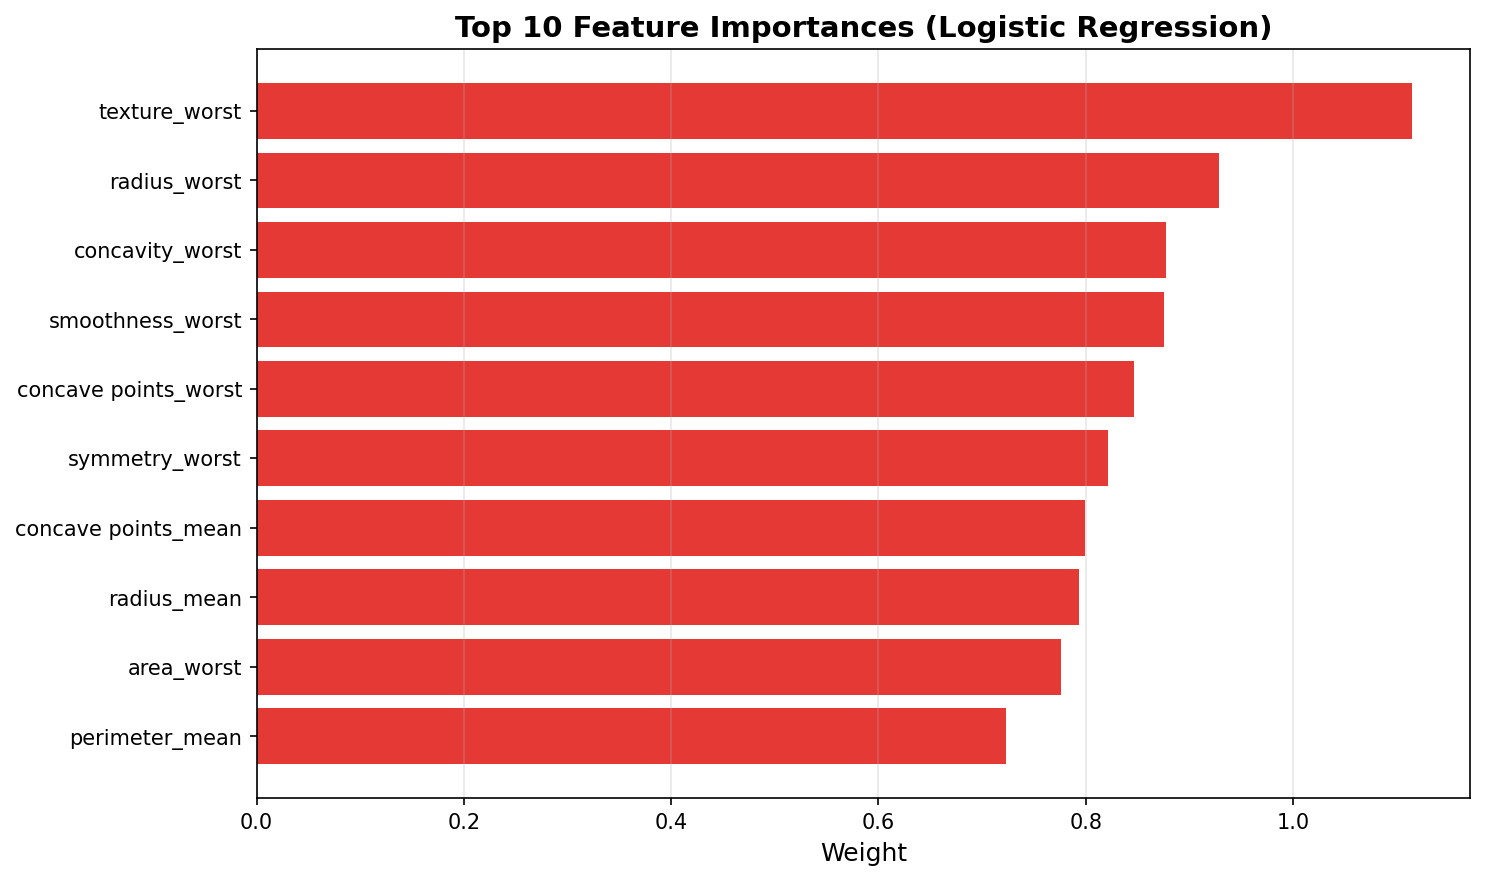
\includegraphics[width=0.75\textwidth]{plots/part1/lr_feature_importance.png}
    \caption{Top 10 feature importances. Red = positive weight (pushes toward malignant), blue = negative.}
    \label{fig:feature_importance}
\end{figure}

\subsection{Decision Boundary}

I retrained a logistic regression model using only the top 2 features (\texttt{texture\_worst} and \texttt{radius\_worst}). Figure~\ref{fig:decision_boundary} shows the result the linear seprator does discriminates between the two classes pretty well though there's some overlap in the middle where both benign and malignant samples coexist.

\begin{figure}[H]
    \centering
    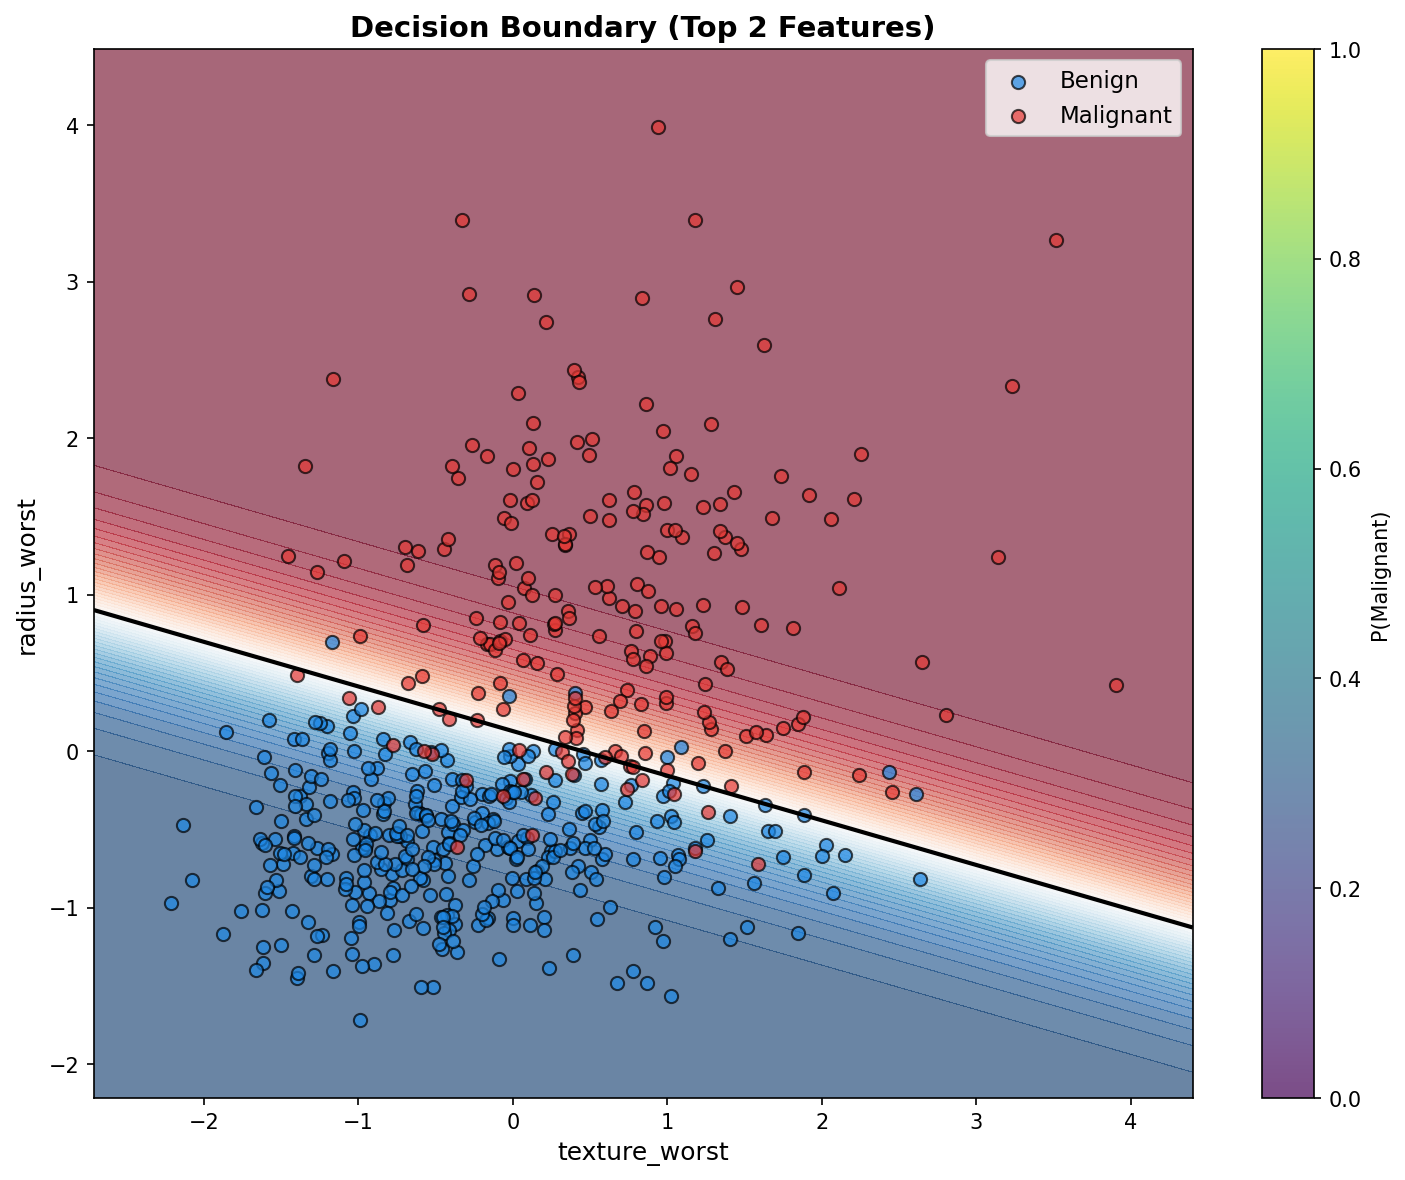
\includegraphics[width=0.75\textwidth]{plots/part1/lr_decision_boundary.png}
    \caption{Decision boundary using the top 2 features. The black line is the 0.5 probability contour.}
    \label{fig:decision_boundary}
\end{figure}

% ============================================================
\section{Multi-Layer Perceptron}
% ============================================================

\subsection{Architectures}

As per part 2, I experimented with three architectures as specified:
\begin{itemize}
    \item \textbf{Linear baseline} (0 hidden layers): This is a single linear layer mapping 30 features to 1 output.
    \item \textbf{Wide network} (1 hidden layer, 100 neurons): Input $\rightarrow$ Linear(30, 100) $\rightarrow$ ReLU $\rightarrow$ Linear(100, 1).
    \item \textbf{Deep network} (3 hidden layers, 10 neurons each): Input $\rightarrow$ [Linear $\rightarrow$ Activation] $\times 3$ $\rightarrow$ Linear(10, 1). This was trained with both ReLU and Sigmoid activations to compare convergence.
\end{itemize}

All models use \texttt{BCEWithLogitsLoss} and SGD with $\alpha = 0.01$ for 1000 epochs. I used the same seed (34) before each model initialization so the comparison is fair.

\subsection{Training Curves}

\begin{figure}[H]
    \centering
    \begin{subfigure}[b]{0.48\textwidth}
        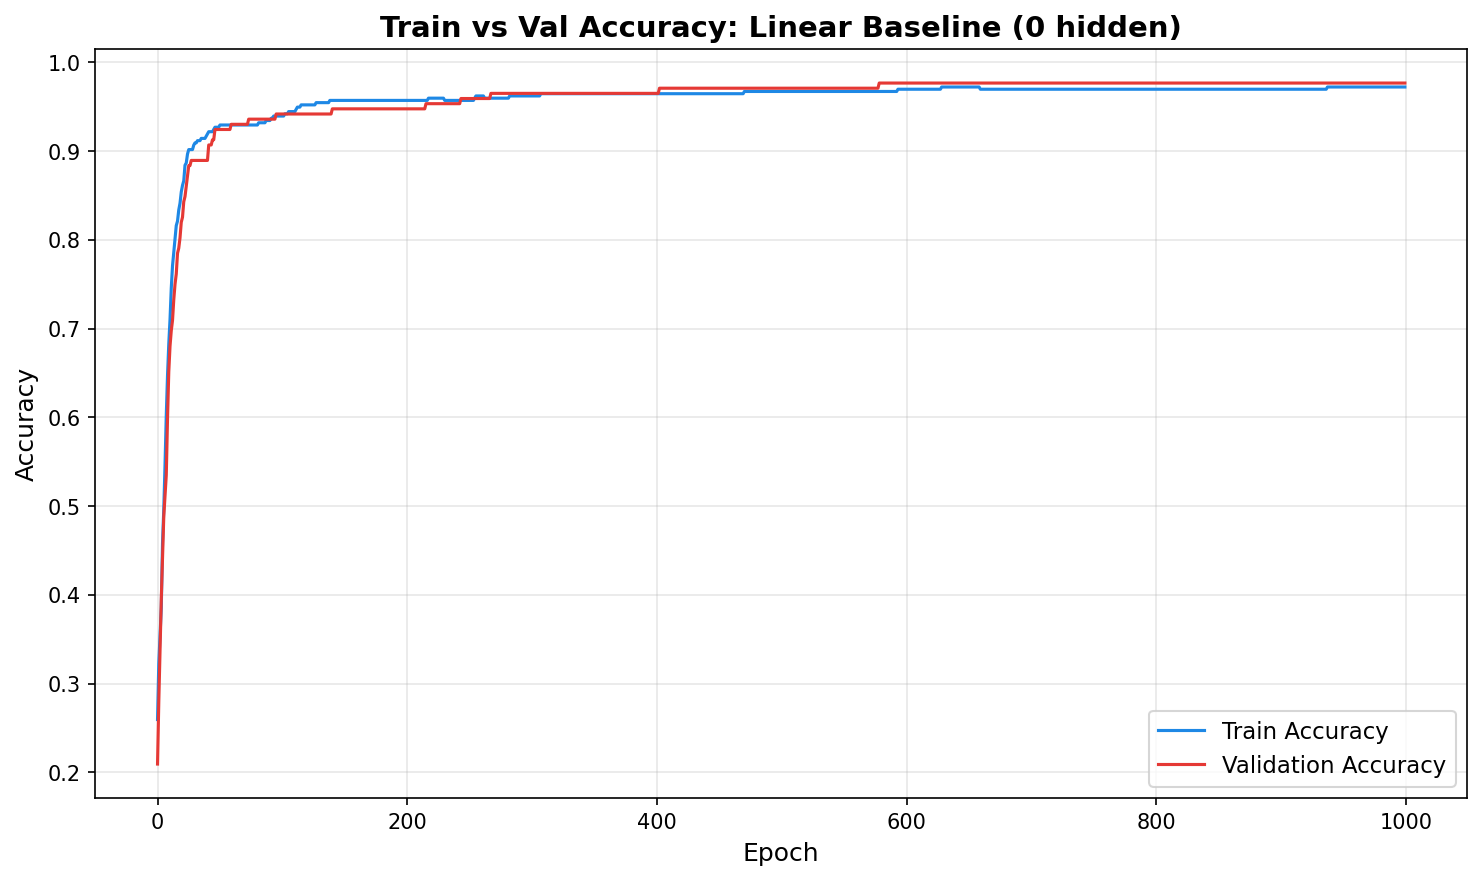
\includegraphics[width=\textwidth]{plots/part2/mlp_train_val_acc_linear_baseline_0_hidden.png}
        \caption{Linear baseline.}
    \end{subfigure}
    \hfill
    \begin{subfigure}[b]{0.48\textwidth}
        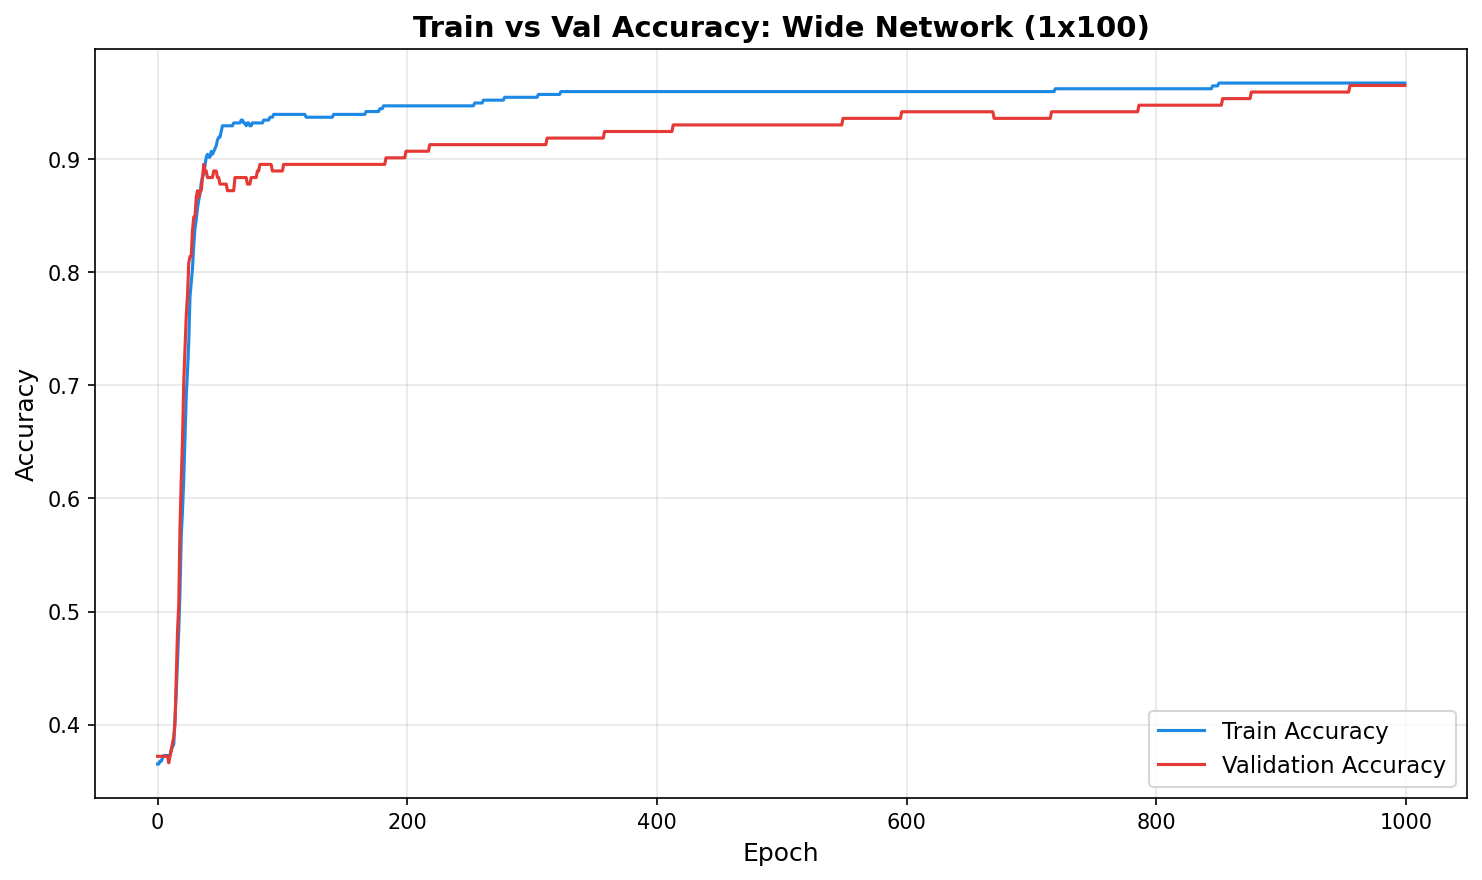
\includegraphics[width=\textwidth]{plots/part2/mlp_train_val_acc_wide_network_1x100.png}
        \caption{Wide network (1$\times$100).}
    \end{subfigure}
    \caption{Training vs.\ validation accuracy for the linear baseline and wide network.}
    \label{fig:mlp_train_val}
\end{figure}

The linear baseline behaves almost identically to the logistic regression from Part~1 which makes sense since it's the same architecture with $\alpha = 0.01$ instead of 0.1. The wide network converges a bit slower but eventually catches up. Neither shows significant overfitting and train and validation accuracy are identical.

The deep network (3$\times$10)  got stuck around 62.8\% accuracy for most of training whic is basically just predicting the majority class (benign) for everything. Maybe because of the initial weights initialization and with SGD at a moderate learning rate, the gradients were probably too small to escape. Hence, the BCE loss stalls after approximately the 150th or 175th epoch.

\subsection{Sigmoid vs ReLU}

\begin{figure}[H]
    \centering
    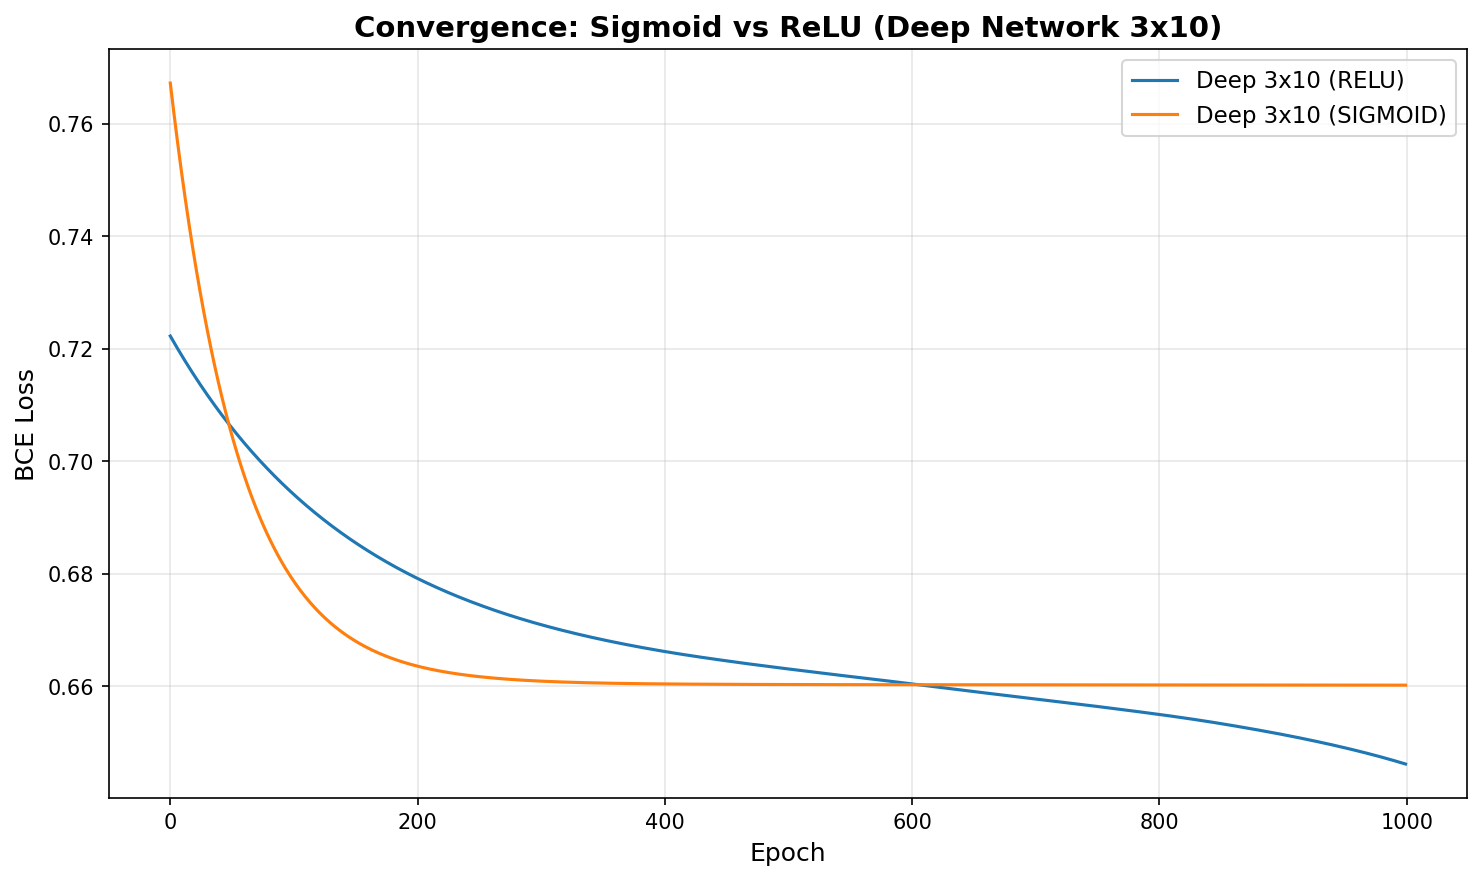
\includegraphics[width=0.75\textwidth]{plots/part2/mlp_sigmoid_vs_relu.png}
    \caption{Convergence comparison: Sigmoid vs.\ ReLU activation in the deep network (3$\times$10).}
    \label{fig:sigmoid_relu}
\end{figure}

Figure~\ref{fig:sigmoid_relu} shows this clearly. The ReLU version at least shows the loss slowly decreasing (from 0.69 to 0.65 over 1000 epochs), so it's making some progress even if it hasn't escaped yet. The Sigmoid version flatlines almost immediately at 0.66. This could be a vanishing gradient problem. With three layers of Sigmoid activations, the gradients get multiplied by $\sigma'(x) \leq 0.25$ at each layer, so by the time they reach the first layer the signal is basically gone.

This is demonstrates why ReLU is a better activation function as compared to sigmoid for deep networks. ReLU's gradient is either 0 or 1, so it doesn't suffer from the same attenuation.

\subsection{Test Set Evaluation}

\begin{table}[H]
\centering
\caption{MLP Test Results (all architectures)}
\label{tab:mlp_results}
\begin{tabular}{lccccc}
\toprule
\textbf{Model} & \textbf{Acc} & \textbf{Prec} & \textbf{Rec} & \textbf{F1} & \textbf{AUC} \\
\midrule
Linear Baseline (0 hidden) & \textbf{0.9767} & 0.9839 & 0.9531 & 0.9683 & 0.9896 \\
Wide Network (1$\times$100) & 0.9651 & 0.9833 & 0.9219 & 0.9516 & 0.9871 \\
Deep Network ReLU (3$\times$10) & 0.6279 & 0.0000 & 0.0000 & 0.0000 & 0.9337 \\
Deep Network Sigmoid (3$\times$10) & 0.6279 & 0.0000 & 0.0000 & 0.0000 & 0.7148 \\
\bottomrule
\end{tabular}
\end{table}

The linear baseline was the best model with 97.67\% accuracy, slightly beating the logistic regression from Part~1 (97.09\%). The wide network is close behind at 96.51\%. The deep networks both fail completely at classification (precision/recall/F1 all zero) because they never learned to predict any malignant cases and they were stuck predicting benign for everything.

Additionally the deep ReLU model's AUC is 0.93 which means the raw logits are actually somewhat ordered correctly even though the threshold-based predictions fail. The model has learned \emph{something} about the data but it just hasn't learned enough to cross the 0.5 decision boundary for any sample.

% ============================================================
\section{Comparative Analysis}
% ============================================================

\begin{table}[H]
\centering
\caption{Full Model Comparison}
\label{tab:comparison}
\begin{tabular}{lccccc}
\toprule
\textbf{Model} & \textbf{Acc} & \textbf{Prec} & \textbf{Rec} & \textbf{F1} & \textbf{AUC} \\
\midrule
Logistic Regression ($\alpha=0.1$) & 0.9709 & 0.9683 & 0.9531 & 0.9606 & 0.9876 \\
Linear Baseline (0 hidden) & \textbf{0.9767} & 0.9839 & 0.9531 & \textbf{0.9683} & \textbf{0.9896} \\
Wide Network (1$\times$100) & 0.9651 & 0.9833 & 0.9219 & 0.9516 & 0.9871 \\
Deep ReLU (3$\times$10) & 0.6279 & --- & --- & --- & 0.9337 \\
Deep Sigmoid (3$\times$10) & 0.6279 & --- & --- & --- & 0.7148 \\
\bottomrule
\end{tabular}
\end{table}

\begin{figure}[H]
    \centering
    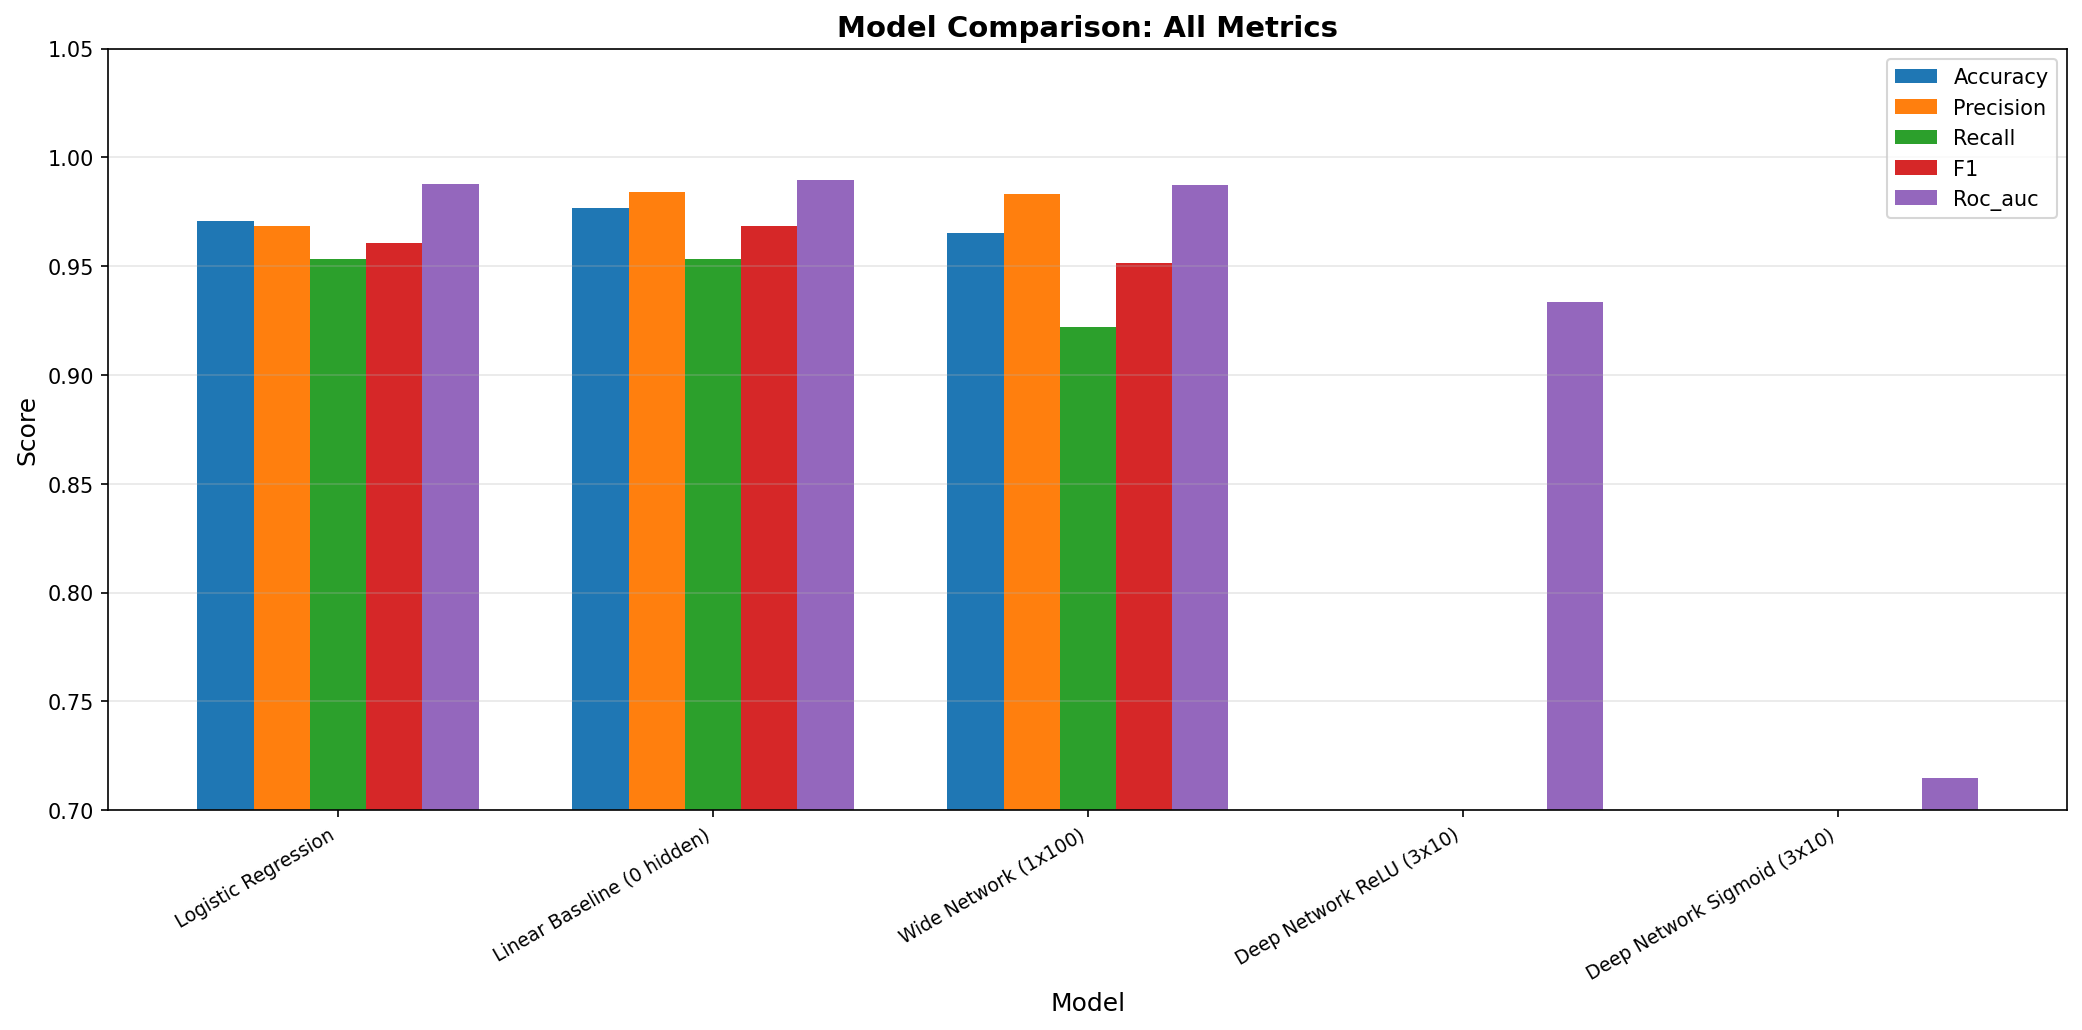
\includegraphics[width=0.85\textwidth]{plots/comparison/model_comparison.png}
    \caption{Metric comparison across all models.}
    \label{fig:comparison}
\end{figure}

The main takeaway is that the MLP doesn't significantly outperform logistic regression on this dataset. The linear baseline (which is architecturally identical to LR) got the best numbers, and adding hidden layers either didn't help (wide network) or actively hurt (deep network). Based on the feature analysis presented we see that the WDBC features were specifically designed to be discriminative, and as the correlation heatmap showed, the classes are nearly linearly separable after standardization.

From a trade-off point of view, logistic regression gives you interpretable weights, runs in seconds, and gets 97\% accuracy. The MLP might provide an extra few percent in accuracy with better tuning, but there is a lose of interpretability which the additional accuracy can't compensate for. For a medical application where doctors need to understand why a model flagged something, the simpler model wins(logisitic regression).

% ============================================================
\section{Assumptions and Notes}
% ============================================================

I went with median imputation over mean because several features are right-skewed (area and perimeter features especially), and medians handle that better. Z-score standardization was required by the assignment, and it's the right choice here anyway since it makes feature weights comparable and helps gradient descent.

I used SGD everywhere rather than Adam. For logistic regression this is fine since the loss surface is convex. For the MLPs, Adam might have helped the deep network escape its bad initialization faster, but the assignment specified SGD so I stuck with it.

The deep network's failure to converge is dependent on the weight initialization at the start. This sensitivity to initialization can be mitigated by trying different initialization schemes , a different optimizer, etc. which was not tried due to a lack of time for this assignment.

% ============================================================
\section{Conclusion}
% ============================================================

Logistic regression got to 97.09\% accuracy with just z-score normalization and gradient descent, and the feature importance analysis pointed to \texttt{texture\_worst}, \texttt{radius\_worst}, and \texttt{concavity\_worst} as the top three features---all clinically meaningful. The MLP experiments showed that adding hidden layers doesn't help on this dataset, and the deep network's convergence issues gave a practical demonstration of why activation function choice and initialization matter. If I had to pick one model for deployment, I'd go with the logistic regression: it's accurate, interpretable, and doesn't have any convergence surprises.

\end{document}
